\chapter{3D Deep Learning}

\section{Deep Learning for 3D Reconstruction}

\subsection{Feature matching}

\subsubsection{Learning to estimation pose}
Using networks to directly predict pose is not good. (不准确且不稳定)

网络的功能之一是记忆, 这个与泛化性相关. 

Use deep learning to improve feature matching. 

\subsubsection{Recap: featrue matching pipline}

\begin{figure}[H]
    \centering
    \begin{tikzpicture}
        \node (a) [rectangle, draw=black]  {Images};
        \node (b) [rectangle, draw=black] [right=1em of a] {Extract Features};
        \node (c) [rectangle, draw=black] [right=1em of b] {Match Features};

        \node [text width=8em] [below= 1em of b] {1.Detection\\ 2.Description };
        \node [below= 1em of c] {3. Matching};

        \draw [->] (a)--(b);
        \draw [->] (b)--(c);
    \end{tikzpicture}
    \caption{Feature matching pipline}
\end{figure}

\subsubsection{Why deep learning}

Traditional feature detectors and descriptors are handcrafted (人工定义) (e.g. DoG, SIFT, ...)

Limitations: Geometry only, no semantics, no semantics, not robust. 

\subsubsection{Deep learning for feature matching}

Example: SuperPoint

\begin{figure}[H]
    \centering
    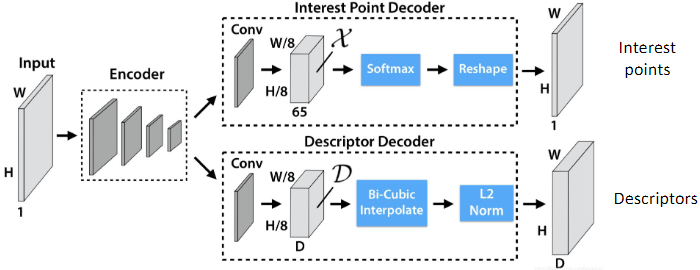
\includegraphics[width=0.618\textwidth]{Lec11/SuperPoint}
    \caption{SuperPoint}
\end{figure}

\begin{enumerate}
    \item CNN-based detectors: Representing feature point locations by heatmaps (热力图).
    
    \begin{figure}[H]
        \centering
        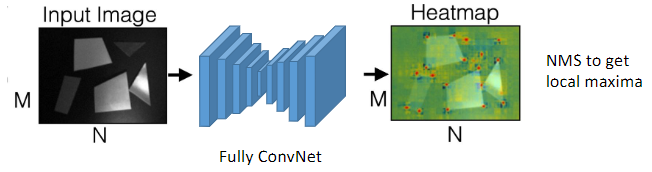
\includegraphics[width=0.618\textwidth]{Lec11/CNN-based detectors}
        \caption{CNN-based detectors}
    \end{figure}

    For training detectors:
    \begin{enumerate}
        \item  Training CNNs to detect corners. 

        \begin{figure}[H]
            \centering
            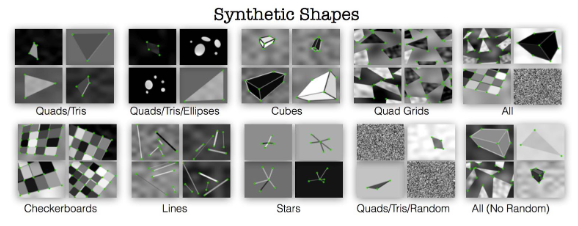
\includegraphics[width=0.618\textwidth]{Lec11/detect corners}
            \caption{detect corners}
        \end{figure}
        \begin{align*}
            L_{loc}=\sum_i \left\| p_t^*-\hat{p}_t \right\|_2
        \end{align*}
        \item Training CNNs to enforce repeatability (不变性)
        
        \begin{figure}[H]
            \centering
            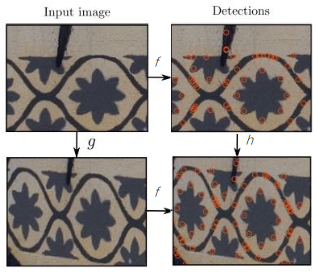
\includegraphics[width=0.218\textwidth]{Lec11/enforce repeatability}
            \caption{enforce repeatability}
        \end{figure}

        \begin{enumerate}
            \item Warp image
            \item Enforce equivariance
        \end{enumerate}
        \begin{align*}
            \min_f \frac{1}{n} \sum_{i=1}^n \left\| f(h(I))-g(f(I)) \right\|^2
        \end{align*}
    \end{enumerate}
    
    \item CNN-based descriptors: Extract descriptors from CNN feature maps. 
    
    \begin{figure}[H]
        \centering
        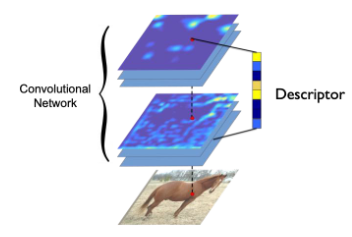
\includegraphics[width=0.318\textwidth]{Lec11/CNN-based descriptors}
        \caption{CNN-based descriptors}
    \end{figure}

    For training descriptors:
    Training descriptors by metric learning
    \begin{figure}[H]
        \centering
        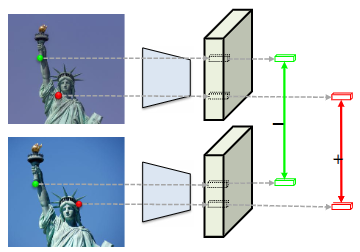
\includegraphics[width=0.3\textwidth]{Lec11/metric learning}
        \caption{metric learning}
    \end{figure}

    \begin{enumerate}
        \item Contrastive loss (最小化对应点距离, 最大化不对应点的距离)
        \begin{align*}
            L_{pos}=& \frac{1}{N} \sum_{i=1}^N \left\| F_I(A)-F_{I^{\prime}}(P) \right\|^2\\
            L_{neg}=&\frac{1}{N}\sum_{i=1}^N \max(0,m-\left\| F_I(A)-F_{I^{\prime}}(N) \right\|)^2 \text{ 取max避免无限制的优化}
        \end{align*}
        \begin{figure}[H]
            \centering
            \begin{subfigure}{0.28\textwidth}
                \centering
                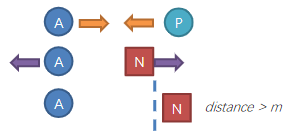
\includegraphics[width=\textwidth]{Lec11/Contrastive loss 1}
            \end{subfigure}
            \begin{subfigure}{0.28\textwidth}
                \centering
                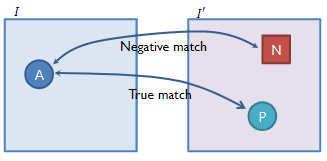
\includegraphics[width=\textwidth]{Lec11/Contrastive loss 2}
            \end{subfigure}
            \caption{Contrastive loss}
        \end{figure}
        
        \item Triplet loss 
        \begin{align*}
            L_{tri}=\frac{1}{N}\sum_{i=1}^N \max(0,m+ \left\| F_I(A)-F_{I^{\prime}}(P) \right\|-\left\| F_I(A)-F_{I^{\prime}}(N) \right\|)^2 \text{ 也同样避免无限制的优化}
        \end{align*}
        \begin{figure}[H]
            \centering
            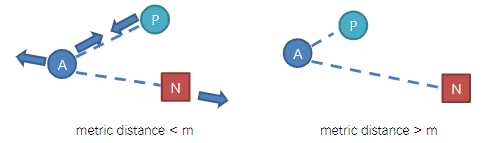
\includegraphics[width=0.618\textwidth]{Lec11/Triplet loss}
            \caption{Triplet loss}
        \end{figure}
    \end{enumerate}
    
    二者效果差不多, 主要是收敛上的差别. 

    Where is training data from? 
    \begin{itemize}
        \item Synthetic data. (但数据不真实)
        \item Use MVS. 
    \end{itemize}
    \begin{figure}[H]
        \centering
        \begin{subfigure}{0.5\textwidth}
            \centering
            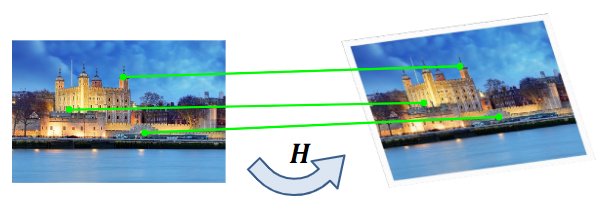
\includegraphics[height=8em]{Lec11/Synthetic data}
            \caption{Synthetic data}
        \end{subfigure}
        \begin{subfigure}{0.3\textwidth}
            \centering
            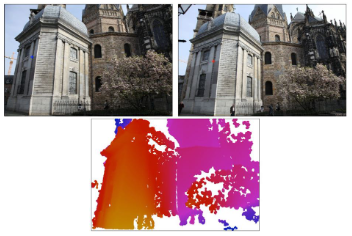
\includegraphics[height=8em]{Lec11/MVS}
            \caption{MVS}
        \end{subfigure}
    \end{figure}
\end{enumerate}

The state of the art is SuperGlue. 

\subsection{Object Pose Estimation}
Estimate the 3D location and orientation of an object realtive to the camera frame. 

\begin{figure}[H]
    \centering
    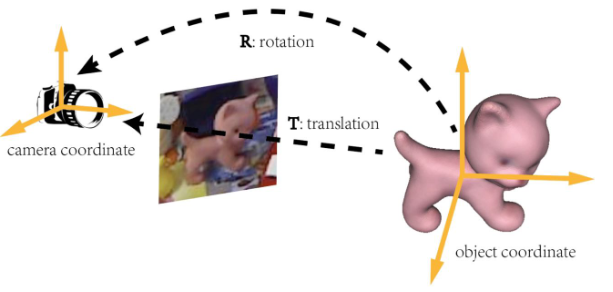
\includegraphics[width=0.618\textwidth]{Lec11/3D location and orientation}
    \caption{3D location and orientation}
\end{figure}

Applications: robot grasping, autonomous driving, augmented reality (AR). 

Similar to visual localization:
\begin{enumerate}
    \item Find 3D-2D correspondences. 
    \item Solve $R$ and $t$ by perspective-n-point (PnP) algorithm. 
\end{enumerate}
\begin{figure}[H]
    \centering
    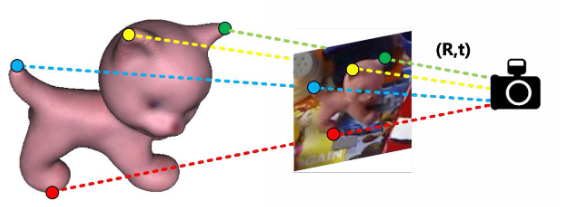
\includegraphics[width=0.618\textwidth]{Lec11/Object Pose Estimation}
    \caption{Object Pose Estimation}
\end{figure}

\subsubsection{Feature-matching-based methods}
\begin{enumerate}
    \item Reconstruct object SfM model by input multi-view images. 
    \begin{figure}[H]
        \centering
        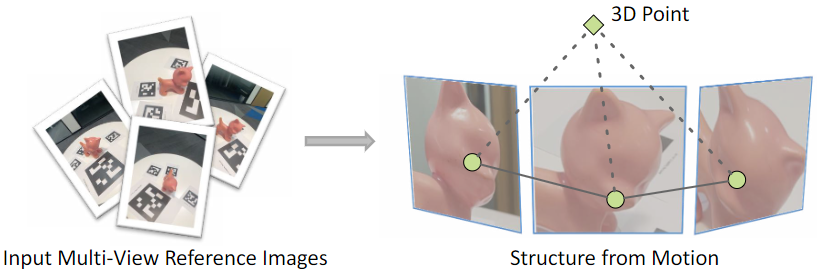
\includegraphics[width=0.618\textwidth]{Lec11/Reconstruct object SfM model}
        \caption{Reconstruct object SfM model}
    \end{figure}
    \item Obtain 2D-3D correspondeces by lifting 2D-2D matches to 3D
    \begin{figure}[H]
        \centering
        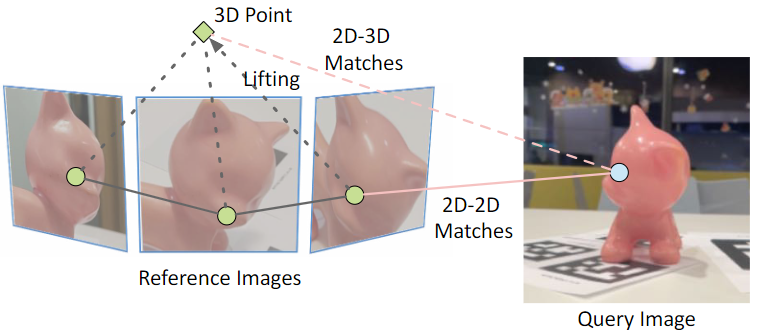
\includegraphics[width=0.618\textwidth]{Lec11/Obtain 2D-3D correspondeces}
        \caption{Obtain 2D-3D correspondeces}
    \end{figure}
    \item Object pose of query image can be solved by PnP.
    \begin{figure}[H]
        \centering
        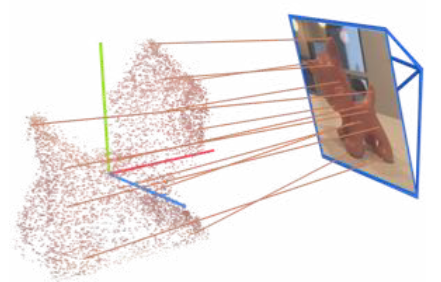
\includegraphics[width=0.3\textwidth]{Lec11/Object pose}
        \caption{Object pose}
    \end{figure}
    \item Futher reading list
    \begin{figure}[H]
        \centering
        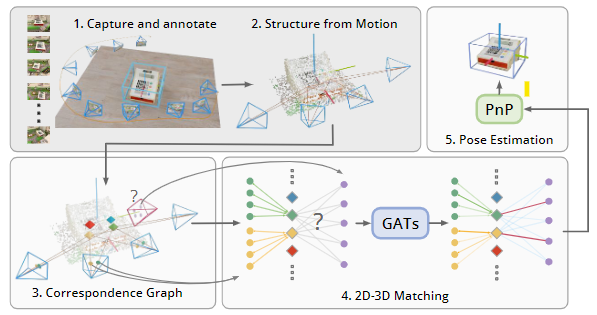
\includegraphics[width=0.618\textwidth]{Lec11/Futher reading list}
        \caption{Futher reading list}
    \end{figure}
\end{enumerate}

\subsubsection{Direct Pose Regression Methods}

Directly regressing object pose of query image using a neural network. Need to render a large amount of images for training.

\begin{figure}[H]
    \centering
    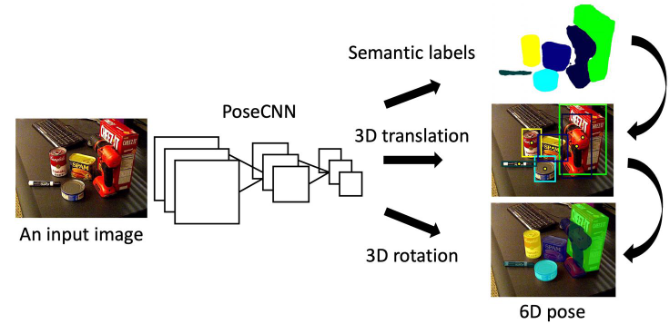
\includegraphics[width=0.618\textwidth]{Lec11/Direct Pose Regression Methods}
    \caption{Direct Pose Regression Methods}
\end{figure}

\subsubsection{Keypoint detection methods}
Using a CNN to detect pre-defined keypoints. Also need to render a large amount of images for training. 
\begin{figure}[H]
    \centering
    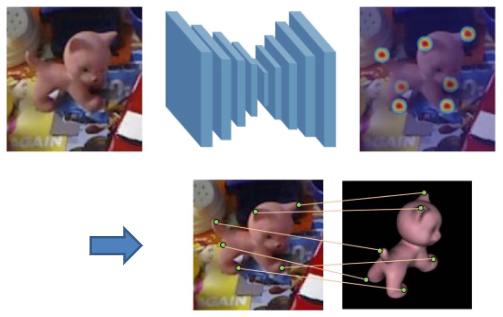
\includegraphics[width=0.418\textwidth]{Lec11/Keypoint detection methods}
    \caption{Keypoint detection methods}
\end{figure}

\subsubsection{Pose refinement methods}

Given estimated pose by above mentioned methods as an initialization. Refine the pose by optimization to obtain more accurate results.

\begin{figure}[H]
    \centering
    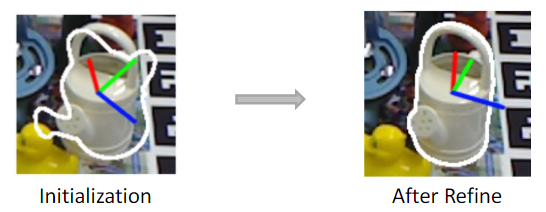
\includegraphics[width=0.418\textwidth]{Lec11/Pose refinement methods}
    \caption{Pose refinement methods}
\end{figure}

\subsection{Human Pose Estimation}
\subsubsection{3D Human Pose Estimation}
\begin{itemize}
    \item 2D Human Pose Estimation: Localize human joints (keypoints – elbows, wrists, etc) in images.
    \item 3D Human Pose Estimation: Estimate a 3D $x, y, z$ coordinate for each joint from image. 
\end{itemize}

\subsubsection{Marker-based MoCap system}
Optical motion capture (MoCap) system. 

\begin{figure}[H]
    \centering
    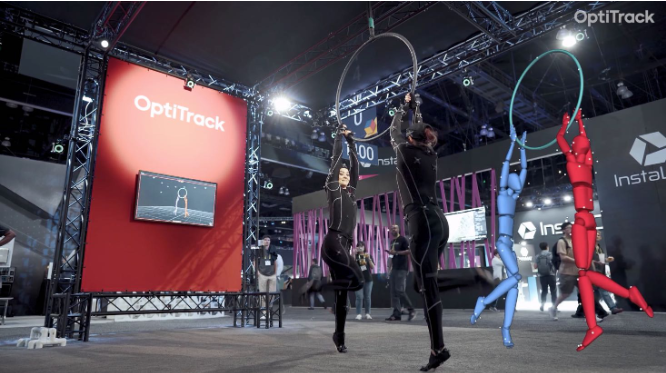
\includegraphics[width=0.318\textwidth]{Lec11/MoCap}
    \caption{MoCap}
\end{figure}

\subsubsection{Markerless MoCap}
Multiview 3D Human Pose Estimation.
\begin{figure}[H]
    \centering
    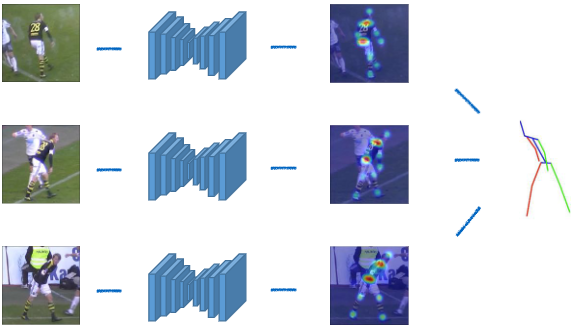
\includegraphics[width=0.618\textwidth]{Lec11/Markerless MoCap}
    \caption{Markerless MoCap}
\end{figure}

\subsubsection{Monocular 3D Human Pose Estimation}
Estimating 3D human pose using a single camera. (如何设计网络, 与如何获取数据, 或者获取人体参数化模型参数, 往往是关节的角度)

\begin{figure}[H]
    \centering
    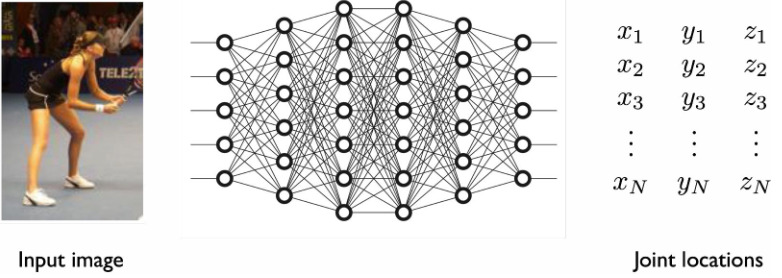
\includegraphics[width=0.618\textwidth]{Lec11/Monocular 3D Human Pose Estimation}
    \caption{Monocular 3D Human Pose Estimation}
\end{figure}

Mehta, Dushyant, et al. "Vnect: Real-time 3d human pose estimation with a single rgb camera."
ACM Transactions on Graphics (TOG) 36.4 (2017): 1-14. 与 https://github.com/mkocabas/VIBE. 

\subsection{Dense Reconstruction}

\subsubsection{Traditional pipeline}
\begin{enumerate}
    \item Compute depth map per image (multi-view stereo)
    \item Fuse the depth maps into a 3D surface (Poisson reconstruction)
    \item Texture mapping
\end{enumerate}

\subsubsection{Recap: multi-view stereo}
Find the depth value that gives the smallest error. 

\subsubsection{Learning MVS}
Challenges for traditional methods: 
\begin{figure}[H]
    \centering
    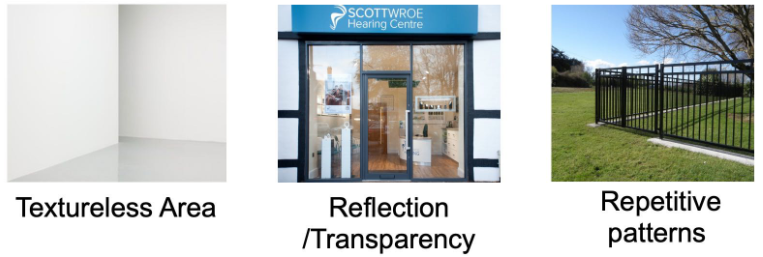
\includegraphics[width=0.418\textwidth]{Lec11/Challenges}
    \caption{Challenges}
\end{figure}

MVSNet: cost volume from CNN features
\begin{figure}[H]
    \centering
    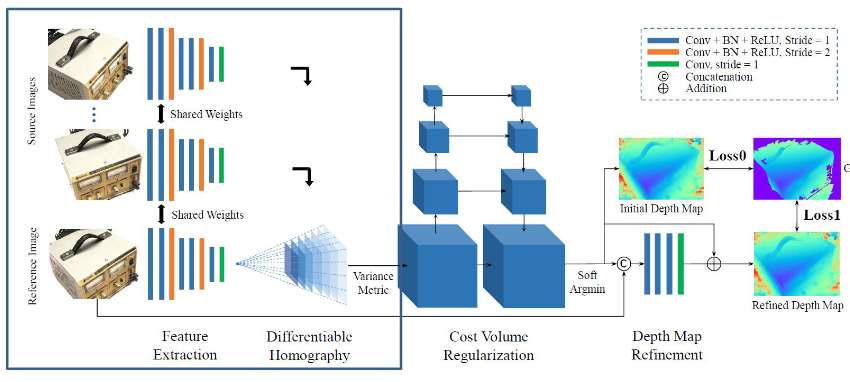
\includegraphics[width=0.618\textwidth]{Lec11/MVSNet}
    \caption{MVSNet}
\end{figure}

Can we improve the mesh quality by comparing the rendered images with the input images?

Yes, but not easy. The rendering process is not differentiable. And mesh representation is not a good representation for optimization. 

\subsection{Single image to 3D}
Infer 3D representation from just single image. (Depth, Point Cloud, Meshm Volume)

\subsubsection{Monoculer depth estimation}
Using network to \textcolor{light_red}{guess} depth from single image. 使用深度摄像机的照片做训练数据. 

\subsubsection{Single-view shape estimation}
3D shape (point cloud, mesh) from a single image. (目前还不是很行, 且单目信息有限, 现训练数据较少)

\section{Deep Learning for 3D Understanding}

\subsection{3D Representations}
Explicit Representations and Implicit Representations
\begin{figure}[H]
    \centering
    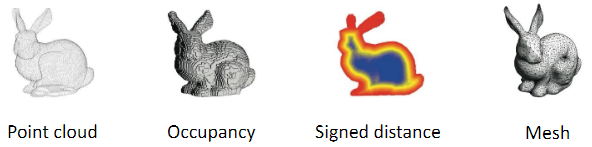
\includegraphics[width=0.618\textwidth]{Lec11/3D Representations}
    \caption{3D Representations}
\end{figure}

\subsubsection{Implicit Representations}
A simple example: $f(p)=1$ represents a sphere where
\begin{align*}
    f(p)=p_1^2+p_2^2+p_3^2
\end{align*}

Generally, the implicit function can be:
\begin{figure}[H]
    \centering
    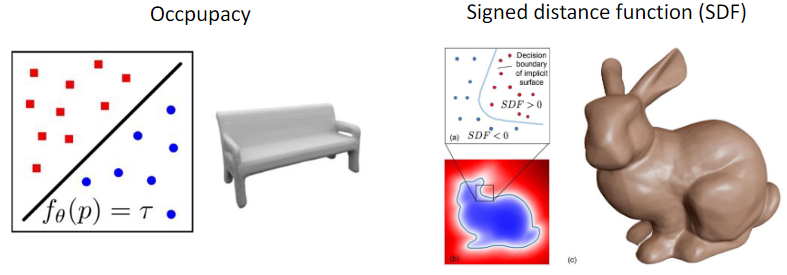
\includegraphics[width=0.618\textwidth]{Lec11/Implicit Representations}
    \caption{Implicit Representations}
\end{figure}

But in practice, the form of $f_{\theta}(p)$ is very hard to define. 

\subsubsection{Implicit Neural Representations}
\begin{figure}[H]
    \centering
    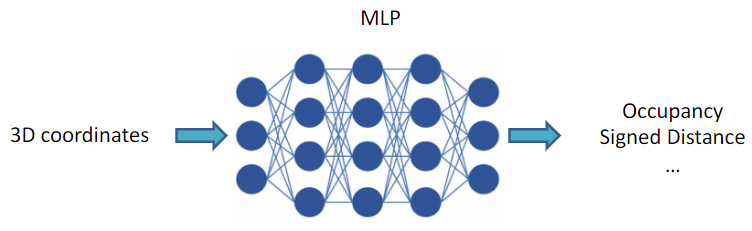
\includegraphics[width=0.618\textwidth]{Lec11/Implicit Neural Representations}
    \caption{Implicit Neural Representations}
\end{figure}

\subsubsection{Neural Radiance Fields (NeRF)}

Representing scenes as radiance fields. 
\begin{figure}[H]
    \centering
    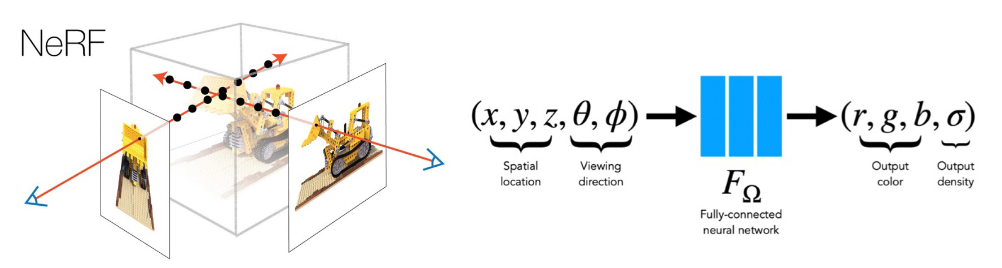
\includegraphics[width=0.618\textwidth]{Lec11/NeRF}
    \caption{NeRF}
\end{figure}

The radiance filed can be converted to images by volume rendering, which is differentiable. 
\begin{figure}[H]
    \centering
    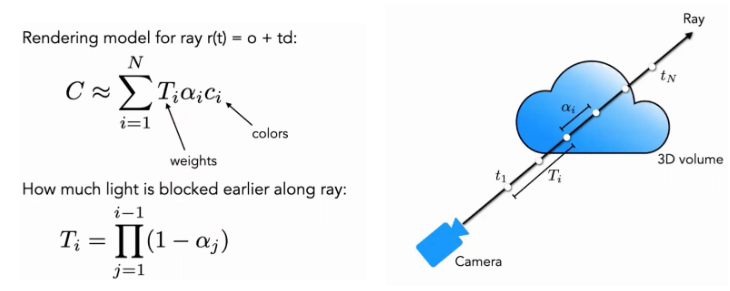
\includegraphics[width=0.618\textwidth]{Lec11/volume rendering}
    \caption{volume rendering}
\end{figure}

Reconstructing NeRF from images by minimizing rendering loss. 
\begin{figure}[H]
    \centering
    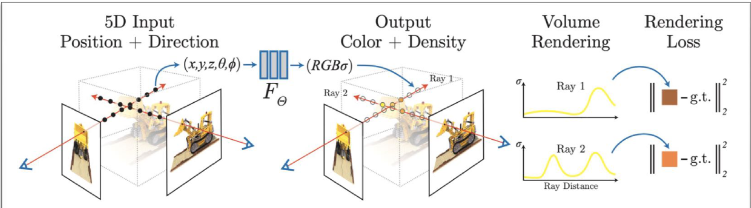
\includegraphics[width=0.618\textwidth]{Lec11/Reconstructing NeRF from images}
    \caption{Reconstructing NeRF from images}
\end{figure}

But NeRF has poor surface reconstruction quality. 

\quad

\quad

\subsubsection{NeuS}

Replacing density field by SDF. 
\begin{figure}[H]
    \centering
    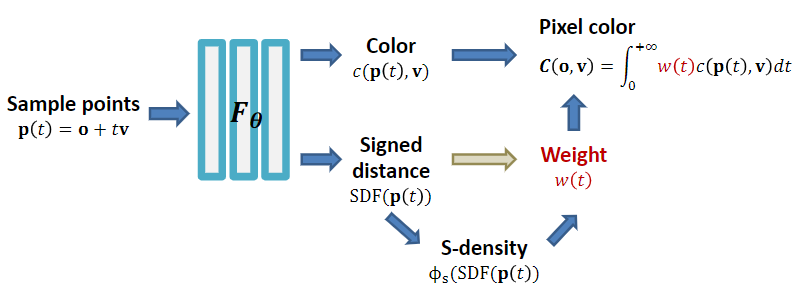
\includegraphics[width=0.618\textwidth]{Lec11/NeuS}
    \caption{NeuS}
\end{figure}

\subsection{3D Classification}
\begin{itemize}
    \item Input: 3D shape
    \item Output: Class
\end{itemize}

\subsubsection{Multi-view CNNs}
\begin{enumerate}
    \item Given an input shape
    \item Render with multiple virtural cameras
    \item The rendered images are passed through CNNs
    \item All image features are pooled and then passed through CNNs
    and to generate final predictions
\end{enumerate}

\begin{figure}[H]
    \centering
    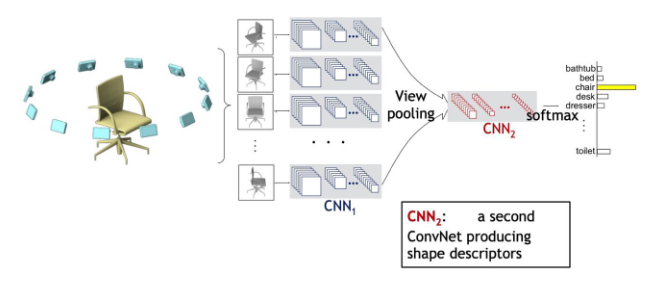
\includegraphics[width=0.618\textwidth]{Lec11/Multi-view CNNs}
    \caption{Multi-view CNNs}
\end{figure}

\subsection{Deep learning on volumetric data}

\subsubsection{3D ConvNets}
Deep learning on volumetric data. Process volumetric data using 3D convlution. 

Challenge: High space/time complexity of high resolution voxels: $O(N^3 )$.

\begin{figure}[H]
    \centering
    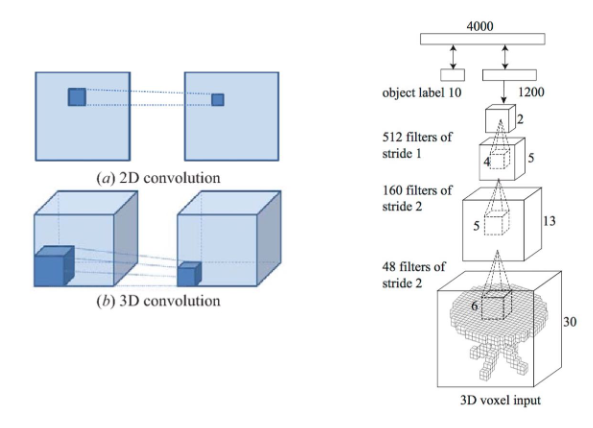
\includegraphics[width=0.518\textwidth]{Lec11/3D ConvNets}
    \caption{3D ConvNets}
\end{figure}

\subsubsection{Sparse ConvNets}
Idea: using sparity of 3D shapes. (三维空间中被占据的部分是比较少的)

\begin{enumerate}
    \item Store the \highlight{sparse} surface signals (Octree, 八叉树)
    \item Constrain the computation \highlight{near the surface}
\end{enumerate}

\begin{figure}[H]
    \centering
    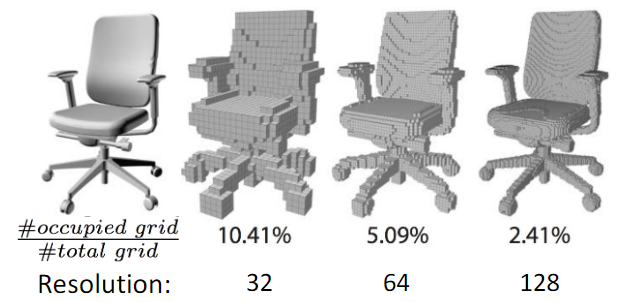
\includegraphics[width=0.418\textwidth]{Lec11/sparity of 3D shapes}
    \caption{sparity of 3D shapes}
\end{figure}

Sparse convolution: compute inner product only at the active sites (nonzero entries)

\begin{figure}[H]
    \centering
    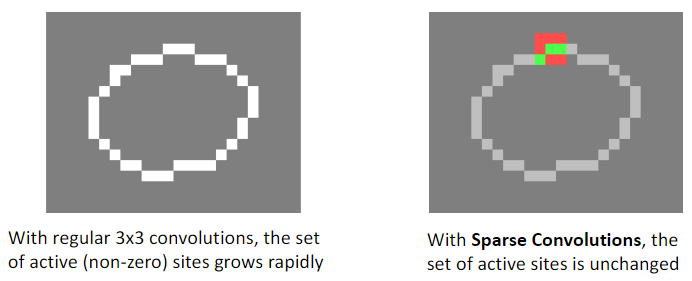
\includegraphics[width=0.418\textwidth]{Lec11/Sparse ConvNets}
    \caption{Sparse ConvNets}
\end{figure}

\subsection{Deep learning on point clouds}
Challenges:
\begin{itemize}
    \item Point cloud is \highlight{unrasterized data (非栅格化)}
    \item Convolution cannot be applied. 
\end{itemize}

\subsubsection{PointNet}

\begin{wrapfigure}[5]{r}{0.38\textwidth}
    \centering
    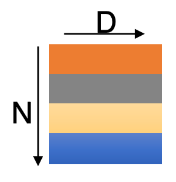
\includegraphics[width=0.1\textwidth]{Lec11/2D array representation}
    \caption{2D array representation}
\end{wrapfigure}

A point cloud processing architecture for multiple tasks (classification, detection, segmentation, registration, etc). 

Point cloud: N orderless points, each represented by a D dim coordinate. 

\quad

\quad

\begin{figure}[H]
    \centering
    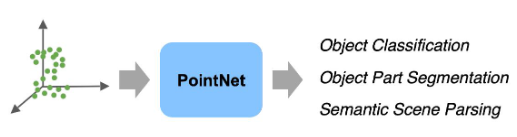
\includegraphics[width=0.618\textwidth]{Lec11/PointNet}
    \caption{PointNet}
\end{figure}

PointNet Classification and Segmentation Architecture. 

\begin{figure}[H]
    \centering
    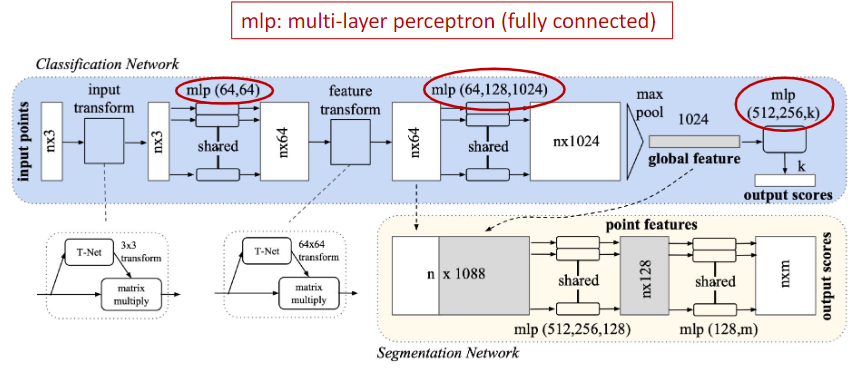
\includegraphics[width=0.618\textwidth]{Lec11/PointNet Network}
    \caption{PointNet Network}
\end{figure}

\begin{enumerate}
    \item Challenge 1: the point set is order-less. The output needs to be invariant to N! permutations. (对点的顺序需要有不变性)
    
    Solution: max pooling makes the output invariant to the order of input points. 
    \item Challenge 2: the output should be invariant to rigid transformation of points. (对模型的位置需要有不变性)
    
    Solution: estimate the transformation using another network (T-Net). 
\end{enumerate}

\subsubsection{PointNet++}
Limitations of PointNet: No local context for each point. 

Three Parts: 
\begin{enumerate}
    \item Sampling: Sample anchor points by \highlight{Farthest Point Sampling (FPS)}
    \item Grouping: Find \highlight{neighbourhood} of anchor points
    \item Apply \highlight{PointNet} in each neighborhood to mimic convolution
\end{enumerate}

\subsection{3D semantic segmentation}

Input: sensor data of a 3D scene (RGB/depth/point cloud .....)

Output: Label each point in point cloud with category label.

Possible solution: directly segmenting the point cloud

\begin{figure}[H]
    \centering
    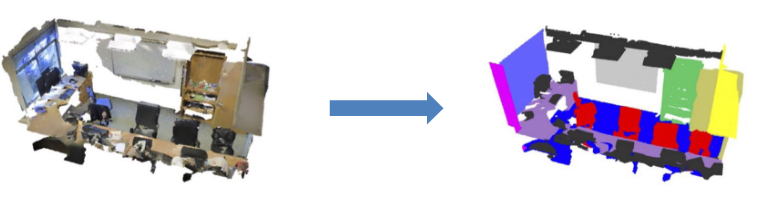
\includegraphics[width=0.618\textwidth]{Lec11/3D semantic segmentation in point cloud}
    \caption{3D semantic segmentation in point cloud}
\end{figure}

Input: sensor data of a 3D scene (RGB/depth/point cloud .....)

Output: Label each point in point cloud with category label.

Possible solution: fuse 2D segmentation results in 3D

\begin{figure}[H]
    \centering
    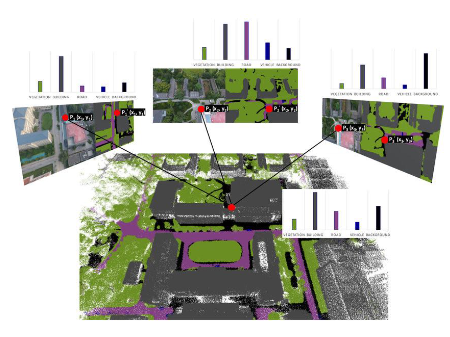
\includegraphics[width=0.418\textwidth]{Lec11/3D semantic segmentation in multi-view}
    \caption{3D semantic segmentation in multi-view}
\end{figure}

\subsection{3D Object Detection}
Detecting 3D objects in 3D data. 

\begin{figure}[H]
    \centering
    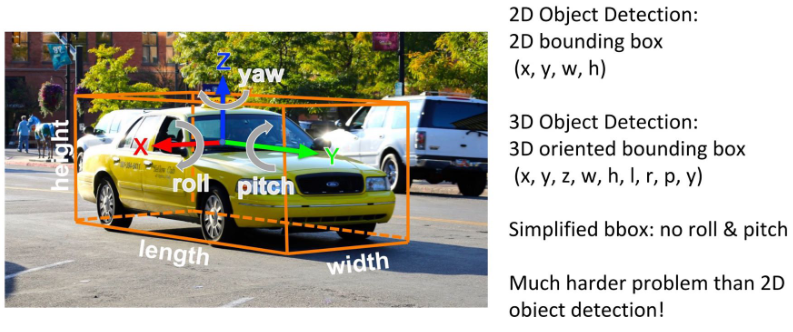
\includegraphics[width=0.618\textwidth]{Lec11/3D bounding boxes}
    \caption{3D bounding boxes}
\end{figure}

\begin{enumerate}
    \item Classify sliding windows. 
    Con: 3D CNNs are very costly in both memory and time. 
    \item PointRCNN: RCNN for point cloud
    \begin{figure}[H]
        \centering
        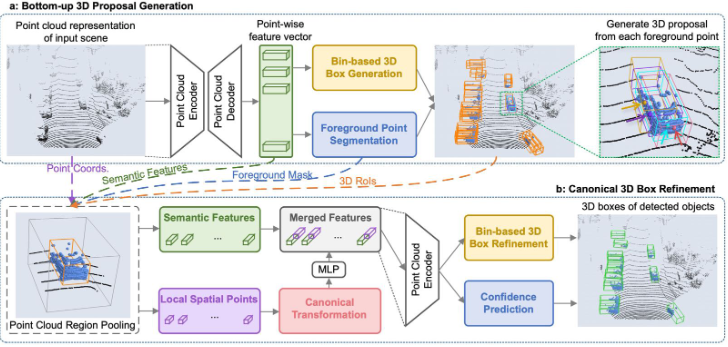
\includegraphics[width=0.618\textwidth]{Lec11/PointRCNN}
        \caption{PointRCNN}
    \end{figure}
    \item Frustum  PointNets: Using 2D detectors to generate 3D proposals. (视锥)
    \begin{figure}[H]
        \centering
        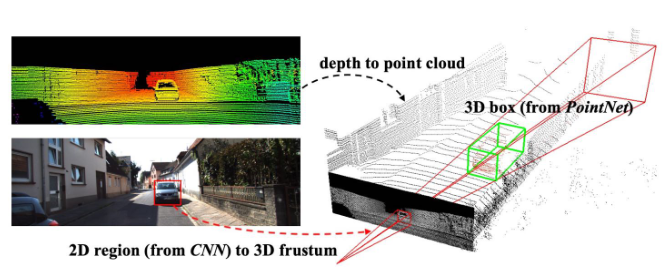
\includegraphics[width=0.618\textwidth]{Lec11/Frustum PointNets}
        \caption{Frustum PointNets}
    \end{figure}
\end{enumerate}

\subsection{3D Instance Segmentation}
Input: 3D point cloud

Output: instance labels of 3D points

\subsubsection{Top-down approach}
\begin{enumerate}
    \item Run 3D detection
    \item Run segmentation in each 3D bbox
\end{enumerate}

\subsubsection{Bottom-up approach}
Group (cluster) points into different objects

\subsection{Datasets for 3D Objects}
\begin{enumerate}
    \item Large-scale Synthetic Objects: ShapeNet
    \item Fine-grained Part: PartNet (ShapeNetPart2019)
    \begin{itemize}
        \item Fine-grained (towards mobility)
        \item Instance-level
        \item Hierarchical
    \end{itemize}
    \item Large-scale Synthetic Scenes: SceneNet
\end{enumerate}

For Out door 3D Scenes
\begin{enumerate}
    \item KITTI: LiDAR data, labeled by 3D bboxes
    \item Semantic KITTI: LiDAR data, labeled per point
    \item Waymo Open Dataset: LiDAR data, labeled by 3D b.boxes
\end{enumerate}